% flashcards-title: Repeated mass readings from two procedures on one shared scale
% flashcards-desc: Two aligned dot plots of mass readings in grams share one horizontal scale from forty-four point six to forty-five point eight grams, with labeled marks every two tenths and small steps at every tenth. The upper row, labeled procedure A, shows four round dots sitting close together near the middle of the scale, two of them stacked at the same value. The lower row, labeled procedure B, shows four diamond-shaped dots spread across a visibly wider stretch of the same scale.
\documentclass[dvisvgm,tikz,border=8pt]{standalone}
\usepackage{tikz}
\usetikzlibrary{arrows.meta,calc,positioning}
\definecolor{DeckInk}{HTML}{172A3A}
\definecolor{DeckAccent}{HTML}{176B87}
\definecolor{DeckWarm}{HTML}{D97706}
\definecolor{DeckMuted}{HTML}{667784}
\definecolor{DeckPaper}{HTML}{F7FAFC}
\tikzset{
  every node/.style={font=\sffamily, text=DeckInk},
  object/.style={draw=DeckInk, line width=1.1pt, fill=DeckPaper},
  primary/.style={draw=DeckAccent, line width=1.5pt},
  boundary/.style={draw=DeckAccent, line width=1.5pt, dashed, rounded corners=6pt},
  guide/.style={draw=DeckMuted, line width=0.9pt, dashed},
  dimension/.style={{Stealth[length=3.2mm,width=2.2mm]}-{Stealth[length=3.2mm,width=2.2mm]}, draw=DeckWarm, line width=1.2pt},
  motion/.style={-{Stealth[length=3.5mm,width=2.5mm]}, draw=DeckAccent, line width=1.5pt, dashed},
}

\begin{document}
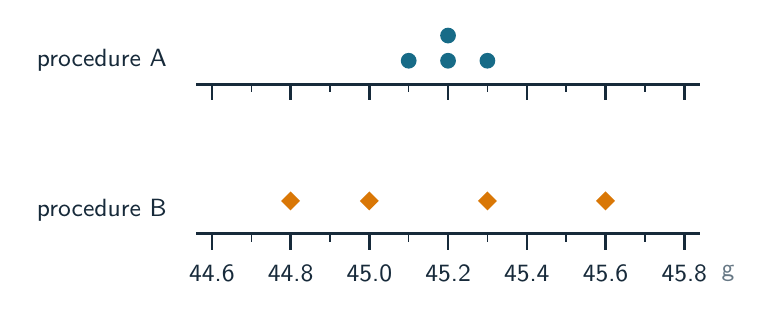
\begin{tikzpicture}[x=1cm,y=1cm]
  % Shared horizontal placement: x = (value - 44.6) * 5
  % Lower axis (procedure B) at y = 0, upper axis (procedure A) at y = 1.9
  \foreach \y in {0,1.9}{
    \draw[DeckInk, line width=1.1pt] (-0.2,\y) -- (6.2,\y);
    \foreach \x in {0,0.5,...,6.0}
      \draw[DeckInk, line width=0.5pt] (\x,\y) -- (\x,\y-0.1);
  }
  \foreach \x/\v in {0/44.6, 1.0/44.8, 2.0/45.0, 3.0/45.2, 4.0/45.4, 5.0/45.6, 6.0/45.8}{
    \draw[DeckInk, line width=0.9pt] (\x,0) -- (\x,-0.2);
    \node[font=\sffamily\small] at (\x,-0.5) {\v};
    \draw[DeckInk, line width=0.9pt] (\x,1.9) -- (\x,1.7);
  }
  \node[font=\sffamily\small, text=DeckMuted, anchor=west] at (6.35,-0.5) {g};
  \node[font=\sffamily\small, anchor=east] at (-0.45,2.2) {procedure A};
  \node[font=\sffamily\small, anchor=east] at (-0.45,0.3) {procedure B};
  % Procedure A readings (circles): 45.1, 45.2, 45.2, 45.3
  \fill[DeckAccent] (2.5,2.2) circle (0.1);
  \fill[DeckAccent] (3.0,2.2) circle (0.1);
  \fill[DeckAccent] (3.0,2.52) circle (0.1);
  \fill[DeckAccent] (3.5,2.2) circle (0.1);
  % Procedure B readings (diamonds): 44.8, 45.0, 45.3, 45.6
  \foreach \x in {1.0,2.0,3.5,5.0}
    \fill[DeckWarm] (\x,0.3) -- (\x+0.12,0.42) -- (\x,0.54) -- (\x-0.12,0.42) -- cycle;
\end{tikzpicture}
\end{document}
